\documentclass{../HM}
\newcommand\course{HM 2}
\newcommand\hwnumber{9}
\usepackage{gauss}
\usepackage{tikz}
\usepackage{pgfplots}

\begin{document}
	\begin{enumerate}
		\item [9.2] In den vier Ecken einer quadratischen Schachtel der Seitenlänge 2 sitzen vier Ameisen, von denen jede in die jeweils im Gegen-Uhrzeigersinn nächste verliebt ist, und daher zu ihr gelangen möchte. Die Ameisen laufen gleichzeitig mit konstanter Geschwindigkeit los, und zwar jeweils auf die von ihr Geliebte zu.
		\begin{enumerate}
			\item Stelle ein lineares System von Differentialgleichungen für die Bahn der Ameisen auf.
			\begin{eqnn}
				\eqntext{Position der Ameise 1:}
				\eqnf{A_1}{\m{x_{11}, x_{12}}}
				\eqntext{Geschwindigkeit der Ameise 1:}
				\eqnf{v_1}{A_2-A_1}
				\eqn{v_1}{\m{x_{21}\\x_{22}}-\m{x_{11}\\x{12}}}
				\eqntext{$A_2 = A_1$ um 90° rotiert $\Rightarrow \m{x_{21}\\x_{22}}=\m{-x_{12}\\x_{11}}$:}
				\eqn[][\Rightarrow]{v_1}{\m{-x_{11}-x_{12}\\x{11}-x_{12}}}
				\eqn[][\Rightarrow]{y}{\m{-1&-1\\1&-1}y}
			\end{eqnn}
			
			\item Bestimme die Bahnkurve der bei $(1,1)$ startenden Ameise.
			\begin{eqnn}
				\eqntext{Eigenwerte und Eigenvektoren bestimmen:}
				\eqn{P_\lambda(A)}{\md{-1-\lambda&-1\\-1&1-\lambda}}
				\eqnf{}{(-1-\lambda)^2+1}
				\eqn{\lambda}{\pm i-1}
				\eqnspace
				\eqn[][\Rightarrow]{\lambda_1}{-1-i,}
				\eqnf{\lambda_2}{-1+i}
				\eqnspace
				\eqn[$v_1$][\Leftarrow]{0}{\m{i&-1\\1&i}[\add[\cdot i][+]{0}{1}]}
				\eqn{0}{\m{i&-1\\0&0}}
				\eqn[][\Rightarrow]{v_1}{\m{-i\\1}}
				\eqnspace
				\eqn[$v_2$][\Leftarrow]{0}{\m{-i&-1\\1&-i}[\add[\cdot(-i)][+]{0}{1}]}
				\eqn{0}{\m{-i&-1\\0&0}}
				\eqn[][\Rightarrow]{v_2}{\m{i\\1}}
				\eqnspace
				\eqn[][\Rightarrow]{y^1}{e^{-(1+i)t}\m{-i\\1},}
				\eqnf{y^2}{e^{(-1+i)t}\m{i\\1}}
				\eqn[][\Rightarrow]{y}{y^1c_1+y^2c_2}
			\end{eqnn}
			\begin{eqnn}
				\eqntext{Anfangswert $y(0)=\m{1\\1}$ einsetzen:}
				\eqn[][\Rightarrow]{\m{-i\\1}c_1+\m{i\\1}c_2}{\m{1\\1}}
				\eqn{\m{-i&i\\1&1}[\add[\cdot(-i)][+]{0}{1}]c}{\m{1\\1}[\add[\cdot(-i)][+]{0}{1}]}
				\eqn{\m{-i&i\\0&2}c}{\m{1\\1-i}}
				\eqn[][\Rightarrow]{c_2}{\frac{1}{2}(1-i)}
				\eqn[][\Rightarrow]{c_1}{\frac{1}{2}(1+i)}
				\eqnspace
				\eqn[][\Rightarrow]{y}{\frac{1}{2}\left((1+i)e^{-(1+i)t}\m{-i\\1}+(1-i)e^{(-1+i)t}\m{i\\1}\right)}
			\end{eqnn}
			\begin{tikzpicture}[remember picture,overlay]
			    \node[xshift=-15mm,yshift=-40mm,anchor=north east] at (current page.north east){
				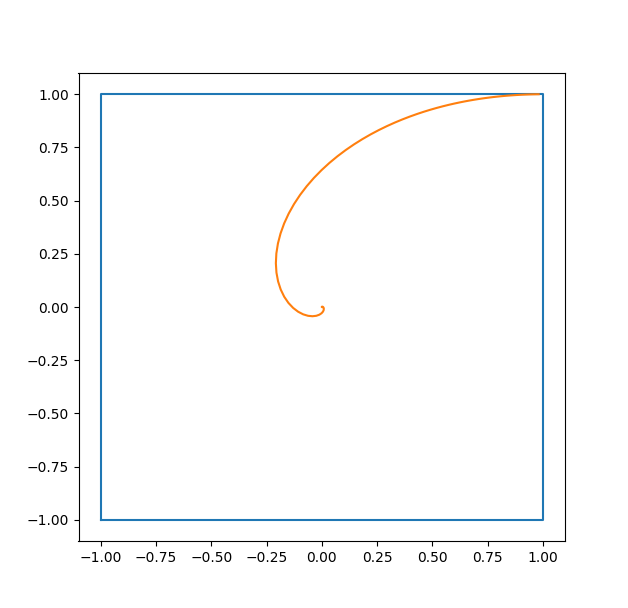
\includegraphics[width=0.4\textwidth]{9.2.png}};
			\end{tikzpicture}
		\end{enumerate}
		
		\item [9.3] Löse das Anfangswertproblem
		$$\begin{cases}
			\dot{y_1}=3y_1+8y_2,&y_1(0)=6,\\
			\dot{y_2}=y_1+y_2+4e^t,&y_2(0)=2.
		\end{cases}$$
		
		\item [9.4] Bestimme eine Lösungsbasis der \textit{Bessel'schen Differentialgleichung der Ordnung} $p=\frac{1}{2}$,
		$$y''+\frac{1}{x}y'+(1-\frac{1}{4x^2})y=0$$,\\
		durch die Substitution $z=y\cdot\sqrt{x}$.
		
		\item [9.5] Betrachtet wird die Differentialgleichung
		$$y'''-3y'+2y=9e^x$$.\\
		\begin{enumerate}
			\item Bestimme eine Lösungsbasis für die zugehörige homogene Differentialgleichung.
			
			\item Finde eine spezielle Lösung durch den Ansatz $y(x)=cx^2e^x$.
			
			\item Löse das Anfangswertproblem zum Anfangswert
			$$y(0)=-1,\quad y'(0)=-8,\quad y''(0)=6$$.
		\end{enumerate}
	\end{enumerate}
\end{document}
